\documentclass[a4paper,11pt]{article}
\input{/home/tof/Documents/Cozy/latex-include/preambule_lua.tex}
\newcommand{\showprof}{show them}  % comment this line if you don't want to see todo environment
\fancyhead[L]{graphe devinette}
\newdate{madate}{10}{09}{2020}
%\fancyhead[R]{\displaydate{madate}} %\today
%\fancyhead[R]{Seconde - SNT}
%\fancyhead[R]{Première - NSI}
\fancyhead[R]{Terminale - NSI}
\fancyfoot[L]{~\\Christophe Viroulaud}
\AtEndDocument{\label{lastpage}}
\fancyfoot[C]{\textbf{Page \thepage/\pageref{lastpage}}}
\fancyfoot[R]{\includegraphics[width=2cm,align=t]{/home/tof/Documents/Cozy/latex-include/cc.png}}
\usepackage{tikz}
\usetikzlibrary{shapes.multipart}
\begin{document}
\begin{Form}
\begin{center}
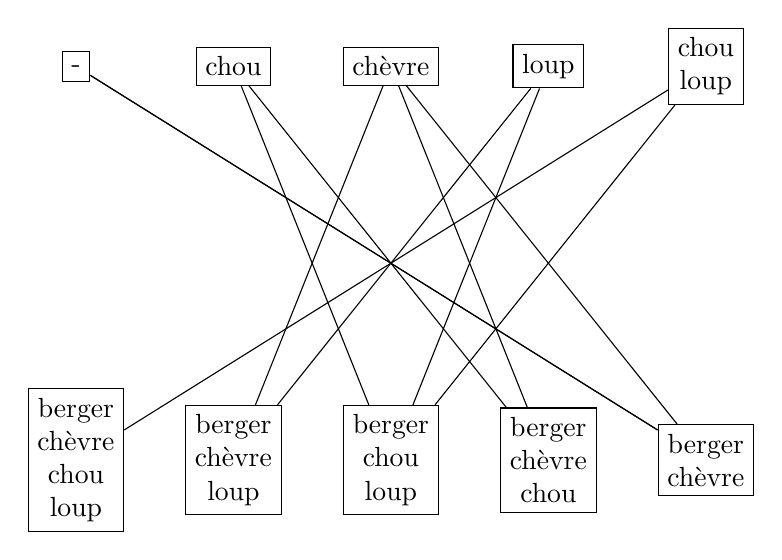
\begin{tikzpicture}[every text node part/.style={align=center}]
\node[draw] (A)at(-4,5) {-};
\node[draw] (B)at(-2,5) {chou};
\node[draw] (C)at(0,5) {chèvre};
\node[draw] (D)at(2,5) {loup};
\node[draw] (E)at(4,5) {chou \\ loup};
\node[draw] (F)at(-4,0) {berger \\ chèvre \\ chou \\ loup};
\node[draw] (G)at(-2,0) {berger \\ chèvre \\ loup};
\node[draw] (H)at(0,0) {berger \\ chou \\ loup};
\node[draw] (I)at(2,0) {berger \\ chèvre \\ chou};
\node[draw] (J)at(4,0) {berger \\ chèvre};

\draw[-,>=latex] (A) -- (J);
\draw[-,>=latex] (C) -- (J);
\draw[-,>=latex] (C) -- (I);
\draw[-,>=latex] (B) -- (H);
\draw[-,>=latex] (B) -- (I);
%\draw[-,>=latex] (D) -- (F);
\draw[-,>=latex] (D) -- (H);
\draw[-,>=latex] (E) -- (F);
\draw[-,>=latex] (E) -- (H);
\draw[-,>=latex] (A) -- (J);
\draw[-,>=latex] (C) -- (G);
\draw[-,>=latex] (D) -- (G);

\end{tikzpicture}
\captionof{figure}{Exemple de transition}
\label{transition}
\end{center}
\end{Form}
\end{document}